
\section{Derivation of $\mathrm{V}_{cs}$ from $\mathrm{W}$ leptonic branching fraction}
\label{sec:physics:vcs}


The coupling strength between \PW boson and the fermion current is $g$. However, due to the quark mixing, the vertex between  \PW boson and quark current is further scaled by a CMK element \absVij. Namely,
\begin{equation}
    \feynmandiagram [inline=(d.base), small, horizontal=d to b] {
        a[particle=\PGn] -- [fermion] b [dot] -- [fermion] c[particle=\Pe],
        b -- [boson] d [particle=\PW],
    };
    = i g \gamma^{\mu} , \qquad
    \feynmandiagram [inline=(d.base), small, horizontal=d to b] {
        a[particle=\(\PQq_j\)] -- [fermion] b [dot] -- [fermion] c[particle=\(\PQq_i\)],
        b -- [boson] d [particle=\PW],
    };
    = i g \absVij.
\end{equation}

\noindent Denoting the partial width of\PW decaying into one generation of lepton current as $\Gamma_\ell$, the tree-level calculation gives
\begin{equation}
    \Gamma_\ell \equiv \Gamma_{\PW \to \ell \PGn} =  \frac{g^2 m_W}{48 \pi} .
\end{equation}


\noindent The NLO electroweak correction of $\Gamma_\ell$ is at $10^{-5}$ relatively level~\cite{dEnterria:2020cpv}, small enough to neglect. The hadronic\PW width decaying into $q_i,q_j$ at the leading order of QCD can be expressed in terms of  $\Gamma_\ell$
\begin{equation}
    \Gamma_{\PW \to \PQq_i \PQq_j}^{\rm LO} = 3 \absVij^2 \frac{g^2 m_W}{48 \pi}  = 3 \absVij^2 \Gamma_\ell ,
\end{equation}


\noindent  where the factor 3 accounts for the three colors. The ratio between the total hadronic and the total leptonic\PW width, at the leading order of \alpS, then equals to the square sum of the CKM elements in the first two rows:
\begin{equation}
    \frac{\Gamma_{\rm had}^{\rm LO}}{\Gamma_{\rm lep}} = \frac{\sum_{ij=(uc)(dsb)} \Gamma_{\PW \to \PQq_i \PQq_j}^{\rm LO} }{ \sum_{\Pe,\mu,\tau} \Gamma_\ell } = \sumCKM.
\end{equation}




% \subsection{Next-to-leading Order of \alpS}

\begin{figure}
    \centering
    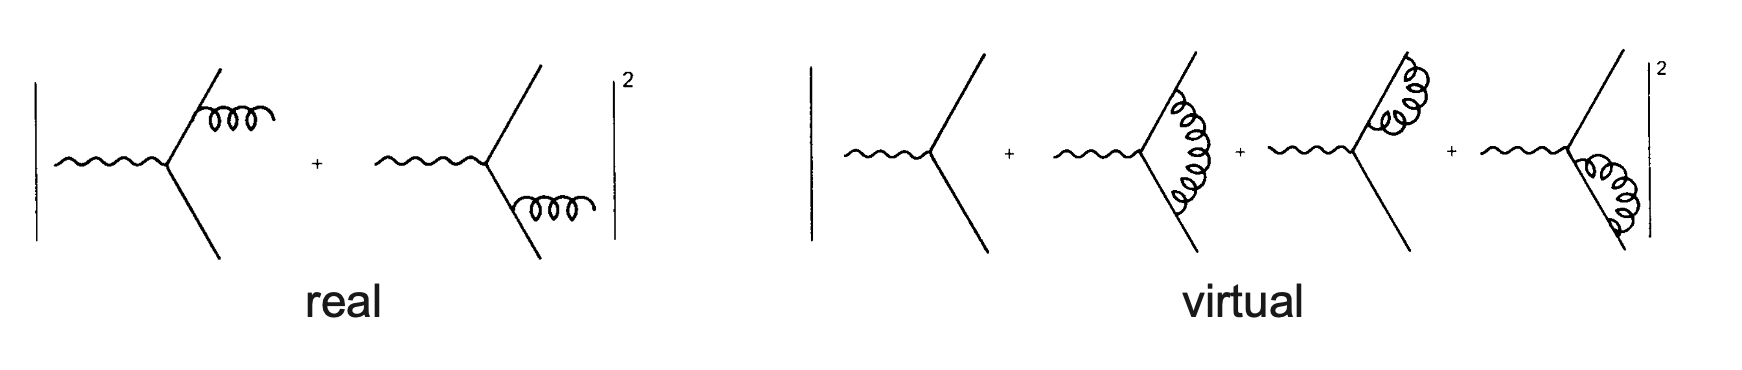
\includegraphics[width=0.8\textwidth]{chapters/Physics/sectionVcs/figures/realVirtual.png}
    \caption{ The real and virtual diagram of\PW decay at the next-to-leading order of \alpS. }
    \label{fig:physics:vcs:realVirtual}
\end{figure}


\noindent At the next-to-leading order (NLO) of \alpS, QCD correction related to the quark current are taken into account. More specifically, the real and virtual diagram shown in Figure~\ref{fig:physics:vcs:realVirtual} add extra contributions to the leading order width $\Gamma_{\PW \to \PQq_i \PQq_j}^{\rm LO} $. The real diagram corresponds to the gluon final state radiation from the outcoming quarks. The virtual diagram corresponds to the interference between the tree level diagram and the virtual gluon bubbles in the quark current and at the vertex. The calculations of the real and virtual contribution can be expressed as a factor multiplied on the tree-level width  $\Gamma_{\PW \to \PQq_i \PQq_j}^{\rm LO} $.
 \begin{align}
 	\Gamma^{\rm V}_{\PW \to \PQq_i \PQq_j}  &= \Gamma_{\PW \to \PQq_i \PQq_j}^{\rm LO} \times \frac{\alpS}{2\pi}\frac{4}{3} \bigg \{  -\ln^2\frac{m_g}{Q} -3 \ln\frac{m_g}{Q} + \frac{\pi^2}{3}-\frac{7}{2} \bigg\} \\
    \Gamma^{\rm R}_{\PW \to \PQq_i \PQq_j}  &= \Gamma_{\PW \to \PQq_i \PQq_j}^{\rm LO} \times \frac{\alpS}{2\pi}\frac{4}{3} \bigg \{  +\ln^2\frac{m_g}{Q} + 3 \ln\frac{m_g}{Q} - \frac{\pi^2}{3}+ 5 \bigg\}
\end{align}
 
\noindent  where $Q$ is the energy of the\PW boson and $m_g=0$ is the mass of the gluon, which makes both the real and virtual width diverge. But the divergences in the real and virtual width exactly cancel each other, leading to a finite total contributions. This QCD correction turns out to be a factor of $k=(1+\frac{\alpS}{\pi})$ :
\begin{equation}
\begin{split}
    \Gamma_{\PW \to \PQq_i \PQq_j}^{\rm NLO} =& \Gamma_{\PW \to \PQq_i \PQq_j}^{\rm LO} + \Gamma^{\rm V}_{\PW \to \PQq_i \PQq_j}  + \Gamma^{\rm R}_{\PW \to \PQq_i \PQq_j}
            =   \Gamma_{\PW \to \PQq_i \PQq_j}^{\rm LO} \big( 1+ \frac{\alpS(M_W)}{\pi}\big)
\end{split} .
\end{equation}

\noindent Therefore at the NLO of \alpS, the ratio between the hadronic and leptonic \PW widths also includes the $k=(1+\frac{\alpS}{\pi})$ factor:
\begin{equation}
    \frac{\Gamma_{\rm had}^{\rm NLO}}{\Gamma_{\rm lep}} =  \underbrace{(1+\frac{\alpS}{\pi})}_{k} \sumCKM. %\sum_{ij=(uc)(dsb)} \absVij^2.
\end{equation}


\noindent For higher order \alpS corrections of the hadronic\PW width, the state-of-art factor has been calculated by considering additional QCD loops. At $\rm N^3LO$, the ratio between the hadronic and leptonic\PW width reads as 
\begin{equation}
    \frac{\Gamma_{\rm had}^{\rm N^3LO}}{\Gamma_{\rm lep}} =   \underbrace{ \bigg [ 1+1.045 ( \frac{\alpS}{\pi} ) + 0.94  ( \frac{\alpS}{\pi} ) ^2 -15  ( \frac{\alpS}{\pi} ) ^3 \bigg ]}_{k} \sumCKM.
\end{equation}

\noindent Finally, the sum square of the CKM elements in the first two rows can be calculated by the experimental measurement of \BWh
\begin{equation}
    \sum_{ij=(uc)(dsb)} \absVij^2 = \frac{1}{k}\times \frac{\BWh }{1- \BWh}
\end{equation}



\noindent where \alpS at the \PW pole can be calculated with $\alpS(\mu_R = m_Z)=0.1178\pm0.0010$~\cite{pdg2020} and the QCD renormalization: $\alpS(m_W) = \alpS(\mu_R) - \alpha^2_s(\mu_R) \frac{ \beta_0}{2\pi} \ln \frac{m_W}{\mu_R} = 0.1199 \pm 0.0010$. The square sum of the five more precisely measured CKM elements can be calculated from the latest experimental results \cite{pdg2020} shown in Table~\ref{tab:physics:vcs:ckm}. $\mathrm{SS_5} = \sumCKMfive = 1.0490 \pm 0.0018$, which leads to the expression for \absVcs:
\begin{equation}
\absVcs = \sqrt{ \frac{1}{k}\times \frac{\BWh }{1- \BWh} - \mathrm{SS_5} } .
\end{equation}


